\chapter{Standard Model}

\label{ch:standardmodel}
% --------------------------------------------------------------------------------

The \ac{SM} of particle physics seeks to explain the symmetries and interactions of fundamental particles. 
The \ac{SM} provides predictions in particle physics for interactions up to the Planck scale (10\tsup{19} \GeV).
It has been tested by several generations of experiments and has been remarkably successful; no significant deviations from its predictions have been found.

The theory itself is a quantum field theory grown from an underlying symmetry, $SU(3) \times SU(2) \times U(1)$, that generates all of the interactions consistent with experimental observations\footnote{excluding gravity}.
These interactions are referred to as the Strong, Weak, and Electromagnetic forces.
Each postulated symmetry necessitates the existence of an associated conserved charge, which appear as properties of the observed particles in nature. 

Although this model has been very predictive, the theory is incomplete; for example, it is not able to describe gravity or astronomically observed dark matter. 
These limitations suggest a need for an extension or new theory to describe physics at higher energies.

%\section{Particles}
%\label{sec:particles}
%
\section{Action and the Lagrangian}

Originally, both action and the Lagrangian were constructed for an integral reformulation of the laws of classical mechanics, which is a purely mathematical step: any differential equation can be re-expressed in terms of an integral equation. 
The Lagrangian, $\mL$, is classically given by the difference of  kinetic energy and potential energy. 
The Lagrangian is defined this way so that the action, $\mS$, given by 
\begin{equation}\label{eq:action}
 \mS[\vect{q}(t)] = \int_{t_1}^{t_2} \mL(\vect{q},\dot{\vect{q}},t)\ dt
\end{equation}
\noindent returns the classical equations of motion when one requires it to be stationary in the path, $\vect{q}(t)$. 
This formulation of classical mechanics is extremely useful in calculations, and generalizes beautifully to cover all types of physics.

In particular, with the development of quantum mechanics in the twentieth century, the concepts of action and the Lagrangian were found to generalize to more complicated physics for which the classical laws do not hold. 
Quantum mechanics and quantum field theory can be constructed from the action, using the path integral formulation, by assuming that a particle undergoes all possible paths $\vect{q}(t)$ with an imaginary phase given by $e^{i \mS[\vect{q}(t)]/\hbar}$. 
This reduces to classical mechanics in the limit as $\hbar$ goes to zero, as all paths for which the action is not stationary interfere with each other so as to cancel their contributions. 
Because the  wavefunction of a particle can be completely determined through the action and the action depends only on the Lagrangian, the Lagrangian itself is sufficient to describe the physics governing the particle. 

So, in both classical and quantum mechanics, the Lagrangian of a system contains everything there is to know about the system, apart from initial conditions. 
Thus, the most natural way to express that a system has a certain symmetry is to require that the Lagrangian is invariant under a corresponding symmetry transformation. 
This makes the Lagrangian the central  piece of the discussion of gauge invariance; the mathematical representation of gauge invariance is that a gauge transformation on the appropriate components of the Lagrangian  returns an identical Lagrangian. 
That is,

\begin{align}
\mL(\psi,D^{\mu}) = \mL(U\psi, D^{'\mu})
\end{align}

\noindent where $\psi$ is the wavefunction and $D^{\mu}$ is the derivative operator, both of which may transform under a symmetry operation.
There are a number of immediate and surprisingly powerful consequences of requiring that the Lagrangian is invariant under a symmetry operation.

\section{Gauge Invariance and Forces}

The simplest possible relativistic, quantum Lagrangian for matter particles is the free Dirac Lagrangian, which describes a relativistic fermion in a vacuum.

\begin{align}\label{eq:free_dirac} 
\mL = i\bar{\psi}\slashed{\partial}\psi -m\bar{\psi}\psi 
\end{align}

\noindent A fermion denotes a particle with spin-1/2, and the kinematic term ($i\bar{\psi}\slashed{\partial}\psi$) is chosen to correctly describe the free propagation of a fermionic particle with mass $m$. 
This equation is invariant under a global $U(1)$ transformation, that is changing $\psi$ by a complex phase has no effect. 
The derivative operator commutes with a constant phase factor, and wherever $\psi$ appears its complex conjugate also appears so as to cancel out the change of phase. 
However, the Lagrangian as written is not invariant under the local $U(1)$ symmetry postulated for the \ac{SM}, which can be written as $U = e^{i\alpha(x)}$. 
The piece of the Lagrangian involving a derivative will return an extra term that will break the invariance of the Lagrangian under this transformation:

\begin{align*}
 \mL' &= i (\bar{\psi}U^\dagger)\slashed{\partial}(U\psi) - m(\psi U^\dagger)(U\psi) \\
      &= i (\bar{\psi}U^\dagger) U(\slashed{\partial} - \gamma^\mu \partial_\mu\alpha(x))\psi - m(\psi U^\dagger)(U\psi) \\
      &= i \bar{\psi}\slashed{\partial}\psi -m\bar{\psi}\psi - i\gamma^\mu \partial_\mu\alpha(x)\bar{\psi}\psi  \\
      &= \mL -  i\gamma^\mu \partial_\mu\alpha(x)\bar{\psi}\psi \\
      &\neq \mL 
\end{align*}

\noindent So, in order to enforce the required symmetry, the typical approach is to construct a covariant derivative, that is to add a term to the derivative operator so that the unwanted term in $\mL'$ is exactly canceled. 
A generic form for such a derivative is given by

\[ D^\mu = \partial^{\mu} - iqA^\mu \]

\noindent where at this point $A^\mu$ is an arbitrary field that transforms under the $U(1)$ operator and $q$ is a scaling factor. Adding this component to the above Lagrangian gives

\begin{align}
 \mL' &=  i (\bar{\psi}U^\dagger) U(\slashed{\partial} - \gamma^\mu \partial_\mu\alpha(x) - iq\gamma^\mu A'_{\mu})\psi - m(\psi U^\dagger)(U\psi) \\
 \mL' &= \mL +\gamma^\mu (- i\partial_\mu\alpha(x) - iqA'_{\mu} + iqA_\mu)\bar{\psi}\psi 
\end{align}

\noindent and because the transformation of $A^\mu$ is unspecified, $\mL = \mL'$ whenever

\[  A'_\mu =  A_{\mu} - \frac{1}{q}\partial_\mu\alpha(x) \]

The above procedure demonstrated that beginning with the Lagrangian for a free fermion and imposing a local $U(1)$ symmetry required the existence of a vector field $A^\mu$, and specified its transformation under the $U(1)$ gauge group.
The additional term in the derivative can be expanded to form a completely separate term in the Lagrangian,

\begin{align}
\mL = i\bar{\psi}\slashed{\partial}\psi -m\bar{\psi}\psi - (q\bar{\psi}\gamma^\mu\psi)A^\mu
\end{align}

\noindent and in this form it is clear that the $A^\mu$ term has the exact form of the electromagnetic interaction.
That is, this is the Lagrangian which reproduces the relativistic form of Maxwell's equations for a particle interacting with an electromagnetic field.
It is natural to also introduce a term to the Lagrangian at this point to describe the free propagation of the vector $A$ field, where the propagation of a vector field has the form of

\begin{align}
- \frac{1}{16\pi} F^{\mu\nu}F_{\mu\nu} \quad \mathrm{with} \quad F_{\mu\nu} = \partial_\mu A_\nu - \partial_\nu A_\mu
\end{align}

\noindent This then also describes the electromagnetic interactions in a vacuum and the propagation of a photon.
This component of the Lagrangian could also potentially include a mass term, but such a term would not be gauge invariant and so must be excluded.
The photon is an example of a gauge boson, a spin-1 particle required to exist by a gauge symmetry of the Lagrangian and one that corresponds to a force.
In summary, requiring the $U(1)$ symmetry was enough to recover all of electromagnetism and to predict the existence of a photon in the \ac{SM}. 

The interaction term that was placed into the Lagrangian by this procedure can be conveniently summarized with Feynman diagrams, which diagrammatically represent a transition from an initial state to a final state.
The contribution of all diagrams that start with the same initial state and end with the same final state must be summed, but more complicated diagrams can be built by linking together the simplest versions.
A diagram that corresponds to the above term, $(q\bar{\psi}\gamma^\mu\psi)A^\mu$, is shown in Figure~\ref{fig:feyn_aff}, for an interaction with a generic fermion.

\begin{figure}
\centering
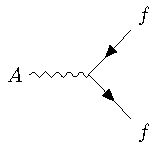
\includegraphics[width=\halffig]{figures/feyn_aff.pdf}
\caption{A Feynman diagram representing the interaction of the $A$ field with a generic fermion, $f$.} 
\label{fig:feyn_aff}
\end{figure}


\subsection{SU(2) $\times$ U(1) and the Electroweak Force}

The full picture of the electroweak section of the \ac{SM} is more complicated than the simplified explanation of the electromagnetic piece described above. 
In practice, it is necessary to consider the entire $SU(2)\times U(1)$ symmetry together, but the procedure is the same.
Enforcing the symmetry on the Lagrangian requires the introduction of a covariant derivative, this time with four total distinct terms, one for each of the generators of $SU(2)\times U(1)$.
The result is a series of terms in the Lagrangian which describe the interaction of a fermion with four vector (spin-1) fields, the $W_1$, $W_2$, $W_3$, and $B$ fields.
These fields can mix in the quantum sense, and linear combinations form the $W^+$, $W^-$, $Z$, and $A$ fields that are considered actual particles in the \ac{SM}\footnote{These states are the actual particles because they are mass eigenstates, but the full explanation of this will have to wait for the discussion of the Higgs mechanism in Section~\ref{sec:higgs_mechanism}.}.

\subsection{$SU(3)$ and the Strong Force}

The same procedure can be applied starting with the $SU(3)$ symmetry requirement, where eight additional fields must be introduced, one for each of the generators of $SU(3)$.
The resulting Lagrangian describes \ac{QCD} and predicts the existence of eight massless gauge bosons known collectively as gluons. 
The complexity of the interactions of those eight gluons leads to surprising phenomena, discussed in Section~\ref{sec:strong}.

\section{Noether's Theorem, Charges, and Matter}

Another direct consequence of the symmetries stipulated in the \ac{SM} are a series of conserved quantities, Noether charges, named after the mathematician and physicist Emmy Noether.
The charges arise as a direct consequence of Noether's theorem, which can be informally stated as 
\begin{quote}
\textit{For every symmetry of the Lagrangian, there exists a corresponding physical quantity whose value is conserved in time.}
\end{quote}
\noindent Or, stated another way, symmetries of the Lagrangian mathematically require the conservation of specific quantities taken from the Lagrangian. 
This relationship can also be thought of as operating in the other direction, the existence of a conserved charge can be shown to generate the symmetry in the Lagrangian.
This theorem is actually quite striking in a somewhat unexpected relation between simple geometric symmetries and physically observable conservation laws. 
For example, the theorem connects the translation invariance of the Lagrangian in space to the conservation of momentum and the translation invariance in time to the conservation of energy. 

In the context of the \ac{SM}, the required symmetries of $U(1)\times SU(2) \times SU(3)$ correspond to the charges that are considered properties of all elementary particles.
The most familiar of these properties is the electric charge, Q, which is one of the conserved quantities of $SU(2)\times U(1)$.
The remaining pieces of $SU(2)\times U(1)$ correspond to weak isospin, $T$ and $T_3$, where $T$ has only non-negative values and $T_3$ can be positive and negative.
$T$ is the magnitude of the full three vector of weak isospin, $\vect{T}$, and $T_3$ is the projection along the third component that is the other conserved quantity derived from $SU(2)\times U(1)$.
The $SU(3)$ symmetry is generated by the three colors of \ac{QCD}, red, green, and blue, each with a corresponding opposite color, anti-red, anti-green, and anti-blue.
The color charges are also conserved in the \ac{SM}.


The matter in the observable universe consists of a collection of particles which carry these charges, in addition to spin and mass.
The matter particles are all fermions: particles with spin-1/2.
All of the fermions belong to one of two groups, quarks and leptons, and one of three generations.
Each of the generations have the same quantum numbers and charges but significantly different masses; the particles in higher generations have increasing mass.
Quarks are distinguished from leptons in that they carry color charge, in addition to  electric charge and weak isospin.
The particles in the \ac{SM} are summarized in Figure~\ref{fig:particle_content}, and the matter particles are the twelve types of fermions displayed on the left side of the graphic.

\begin{figure}[h]
  \centering
  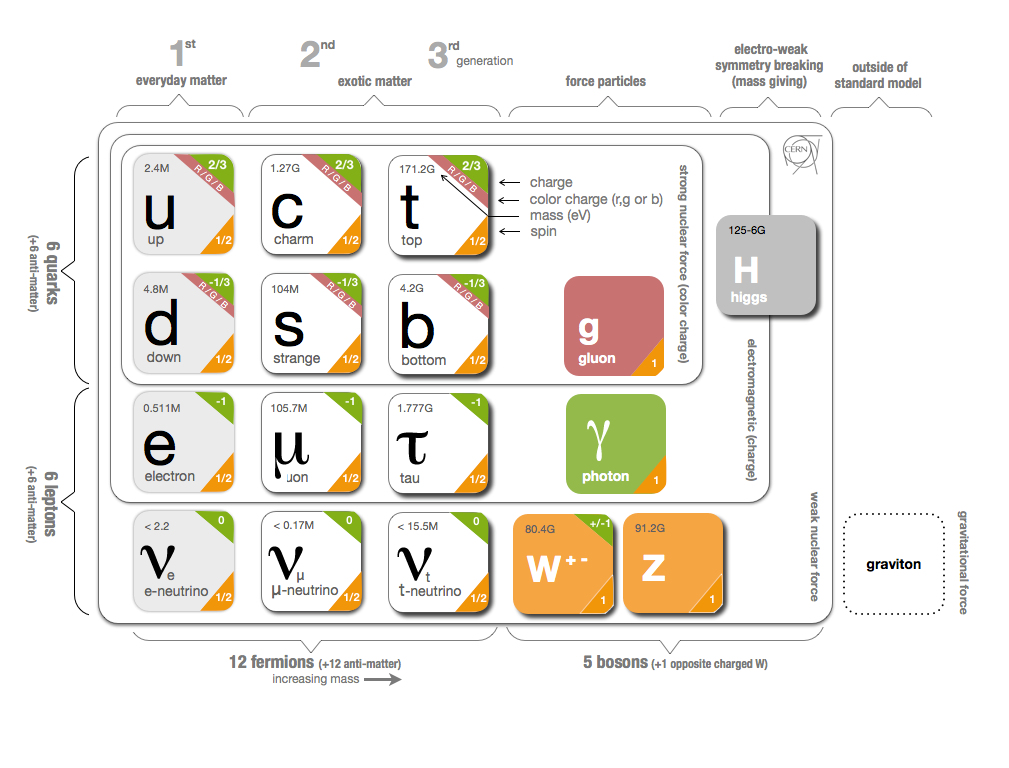
\includegraphics[width=\textwidth]{figures/particle_content.png}
  \caption{The particle content of the \acs*{SM}, including the names, masses, spins, and charges of each of the particles.}
  \label{fig:particle_content}
\end{figure}


\subsection{Quarks}

The three generations of quarks each consist of a quark with electric charge $+2/3$ and one with charge $-1/3$.
They are called up and down, charm and strange, and top and bottom respectively, and these are referred to as the quark flavors.
Although Figure~\ref{fig:particle_content} only shows these six flavors, there is a unique particle for each combination of the three colors and flavor.
And each quark has an anti-particle with the opposite electric charge values.

However, individual quarks are never observed in nature, but instead form color-neutral bound states. 
This is a consequence of interaction of gluons with color charge called confinement, discussed in Section~\ref{sec:strong}.
One way to form a color neutral combination is a bound state of three quarks with three different color charges, called a baryon.
Baryons are the most common type of quark configuration in conventional matter, and include protons and neutrons.
The other common configuration is a bound state of a quark and an anti-quark, called a meson, where the two quarks have opposite colors. 
Although there is no direct conservation law resulting from the symmetries of the \ac{SM} Lagrangian, an accidental symmetry results in the approximate conservation of baryon number, $B$, where baryons have $B=1$ and mesons have $B=0$. That is, no interactions have been observed which directly alter baryon number.

\subsection{Leptons}

The remaining fermions, the leptons, do not carry color charge.
Each generation contains an electrically charged lepton, the electron, muon, and tau, and an electrically neutral lepton called a neutrino.
For the charged leptons, the flavors are mass eigenstates, with the masses listed in Figure~\ref{fig:particle_content}.
The flavors of the neutrinos, on the other hand, are not mass eigenstates: their propagation in quantum superpositions of flavor states leads to oscillations between different flavors.
The absolute masses of the neutrinos are not currently known, but the phenomenon of oscillations shows that they have three different mass values.
Another accidental symmetry leads to an approximate conservation of lepton number $L$, the difference in the number of leptons and anti-leptons; again there are no interactions present in the \ac{SM} which directly alter lepton number.

\subsection{Chirality}

All of the fermions described above have two possible values of the magnitude of weak isospin, $T$, either $0$ or $1/2$.
The fermions with $T = 0$ are called right-handed, while those with $T=1/2$ are called left-handed.
Because $T$ is the charge corresponding to the weak force, right-handed particles do not interact with the weak gauge bosons in the same way that neutral particles do not interact with photons.
For left-handed fermions, each of the quark and lepton generations have one particle with $T_3 = -1/2$ and one with $T_3 = +1/2$.
The neutrinos have $T_3 = +1/2$, while the charged leptons have $T_3 = -1/2$.
Similarly, the positively charged quarks have $T_3 = +1/2$ and the negatively charged quarks have $T_3 = -1/2$.
Because the right-handed neutrinos would have no charge of any type, it is not clear if they exist at all.


\section{Higgs Mechanism and Mass}
\label{sec:higgs_mechanism}

The description of the electroweak forces above left out an important part of the observed nature of the electroweak force.
Many physical experiments observed phenomena corresponding to the interaction of the weak bosons that were best explained if they had significant masses.
But as mentioned before, massive bosons would break the gauge invariance of the Lagrangian.
A large mass for the W and Z bosons is necessary to explain the relative weakness of their interactions compared to the electromagnetic field.
The Lagrangian's discussed above did not include a mass term for the gauge bosons, and in fact such a term would not be allowed by the requirement of gauge invariance. 
This was a significant problem for the \ac{SM}, and the symmetry of the electroweak sector would have to be broken in order to allow for non zero masses for some of the gauge bosons.

One mechanism to allow for this symmetry breaking is the Higgs mechanism, which posits the existence of an additional scalar field.
It begins with a $SU(2)\times U(1)$ invariant Lagrangian of the form 

\begin{equation}
  \mL = |D_\mu\phi|^2 - \frac{1}{2}\mu^2\phi^+\phi - \frac{1}{4}\lambda(\phi^+\phi)^2
\end{equation}

\noindent where $\phi$ is the new scalar field with two components and, importantly, $\mu^2$ is negative.
This leads to a minimum value of the field at a non-zero value of $\phi$, specifically where

\begin{equation}
 \langle \phi \rangle = \frac{1}{\sqrt{2}} \begin{pmatrix}0\\v\end{pmatrix} \quad \mathrm{with} \quad v = \frac{2\mu^2}{\lambda}
\end{equation}

\noindent Expanding the original Lagrangian about its expectation value in terms of the perturbation $H$,

\begin{equation}
  \langle \phi \rangle = \frac{1}{\sqrt{2}} \begin{pmatrix}0\\v + H\end{pmatrix}
\end{equation}

\noindent gives potential terms in the Lagrangian like 

\begin{equation}
  \mL_{H} = -\frac{1}{2}m_H^2 H^2 - \sqrt{\frac{\lambda}{2}}m_H H^3 - \frac{1}{4}\lambda H^4
\end{equation}

\noindent where $m_H = \sqrt{2}\mu$.
The form of this Lagrangian shows that the non-zero expectation value of the $\phi$ field has introduced a massive scalar field $H$ with self interaction terms.
It has an additional important consequence on the description of the gauge bosons, through the expansion of the term involving the covariant derivative:

\begin{equation}
  |D_\mu\phi|^2 \supset \frac{1}{8}\left(g^2(W_{1\mu}W_1^\mu + W_{2\mu}W_2^\mu) + (g'B_\mu - gW_3{\mu})^2\right)
\end{equation}

where the $W_i$ and $B$ fields are the original $SU(2)\times U(1)$ gauge fields mentioned previously.
The above equation can be rearranged using linear combinations of the fields to form mass terms for the gauge bosons, and the mass eigenstates are exactly the $W^\pm$, $Z$, and $A$ fields.
Only the $A$ field, corresponding to the photon, results in a zero mass, and the remaining three particles have non-zero mass values.
Because the previously introduced Lagrangian, written in terms of $\phi$, was clearly gauge invariant, this resulting configuration must also be gauge invariant.

This is the Higgs mechanism, where the introduction of a gauge invariant scalar field with a non-zero expectation value can generate masses for the gauge bosons without violating the underlying symmetries.
The particle that is associated with the perturbations of this field, $H$, is called the Higgs boson, and is said to generate the masses of the remaining bosons because the vacuum expectation value introduces mass-like terms for each of the bosons.
The resulting masses are listed in Figure~\ref{fig:particle_content}.
Because this mechanism was so successful in describing the observed properties of the $W$ and $Z$ bosons, it has been considered part of the \ac{SM} for decades, although the actual Higgs boson was only recently observed in 2012, fully confirming the theory.

The Higgs mechanism is also responsible for generating the masses of the fermions.
The original mass terms that were listed in the Lagrangian for fermions are replaced with Yukawa coupling terms, which introduce interactions between the $\phi$ field and the fermions.
Like with the gauge bosons, the non-zero expectation value of the field yields mass terms, and the expansion about that value introduces interaction terms between the fermions and the Higgs boson.
The masses are different between each fermion because each has a different Yukawa coupling, which results in the masses listed in Figure~\ref{fig:particle_content}.

\section{Phenomenology}

The \ac{SM} Lagrangian described above contains all of the information necessary to describe particle physics through the path integral formulation. 
However, a tremendous amount of complexity emerges from that description because of the diverse allowed interactions between the ensemble of particles in the \ac{SM}.
A qualitative understanding of the phenomenology produced by those interactions is immensely helpful in understanding the analysis of particle physics.

\subsection{Standard Model Calculations}
\label{sec:smcalc}

The terms in the Lagrangian describing interactions of particles can be used to evaluate cross sections or decay widths through perturbation theory.
A cross section quantifies the probability of a given process to result in a scattering of particles, measured as an effective area, while a decay width measures the width of the mass distribution of a particle, which is inversely proportional to its lifetime.
Perturbation theory uses a diagrammatic expansion to approximate \ac{SM} interactions as a series of feynman diagrams, each representing an amplitude for the transition between initial and final state.
The feynman diagrams uniquely specify that transition amplitude through the feynman rules~\cite{peskin}.
The transition amplitude includes a phase space component to account for the initial and final momenta, and an addition matrix element which describes the interaction.
The complex amplitude for each process with the same initial and final state must be summed, and then the cross section or decay width is calculated as the square of the amplitude integrated over all valid final state momenta.
For example, the decay rate for a particle of mass $m_A$ to two final state particles with momenta $\vect{p}_i$ and $\vect{p}_j$ is given by

\begin{align*}
\Gamma = \int \frac{d^3p_i d^3 p_j}{(2\pi)^6 4E_i E_j} (2\pi)^4 \delta^{(4)}(\vect{p_A} - \vect{p_i} - \vect{p_j})\ |\mathcal{M}|^2 
\end{align*}

\noindent where the prefactor is the phase space term, the delta function enforces conservation of four-momentum, and $\mathcal{M}$ is the matrix element.
The matrix element includes dimensionless constant terms that describe the strength of the interaction, called coupling constants: $\alpha$ for the photon, $\alpha_W$ for the weak bosons, and $\alpha_s$ for the gluons.

The sum over all diagrams with the same initial and final state leads to important consequences in the \ac{SM}.
Most process have a small number of leading order diagrams, where leading order indicates the diagram with the fewest factors of the coupling constants.
When the coupling constants are less than unity, the diagrams of higher order have diminishing contributions.
This is called the perturbative regime, and allows for approximate calculations by using a set order, referred to as \ac{LO}, \ac{NLO}, and so on.
A coupling constant greater than unity results in a non-perturbative regime, and requires other calculation techniques.

However, even in a perturbative theory, the sum over all diagrams in the amplitude includes loop diagrams; for example any photon line in a feynman diagram can be replaced with the line in Figure~\ref{fig:loop_diagram} and still form a vaild interaction.
These and other types of loop diagrams introduce divergent contributions to \ac{SM} processes, which would seem to make the theory inconsistent.
The solution to this problem is to absorb those contributions into the coupling constants and charges in the Lagrangian, so that the combination of the bare value and the loop contributions gives the correct physical observables.
This process is called renormalization, and a theory where the divergences can consistently be absorbed into the definition of the constants in the Lagrangian is called renormalizable.

\begin{figure}
\centering
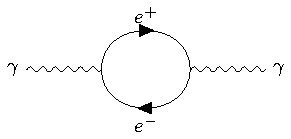
\includegraphics[width=\halffig]{figures/loop.pdf}
\caption{A feynman diagram for photon propagation including a loop of electrons.}
\label{fig:loop_diagram}
\end{figure}

Setting the renormalized coupling constants requires a measurement at a specific energy scale, and only at that scale are the contributions of the loop diagrams precisely cancelled.
At a different energy the loop diagram contribution changes, and can be though of as a modification to the coupling constant.
The renormalization procedure thus predicts a variation of the coupling constants with the scale of the interaction, and specifies how they change with energy.
The energy dependence is called the running of the coupling constants, and the effect on the three couplings in the \ac{SM} is shown in Figure~\ref{fig:unification_sm}.

\begin{figure}
\centering
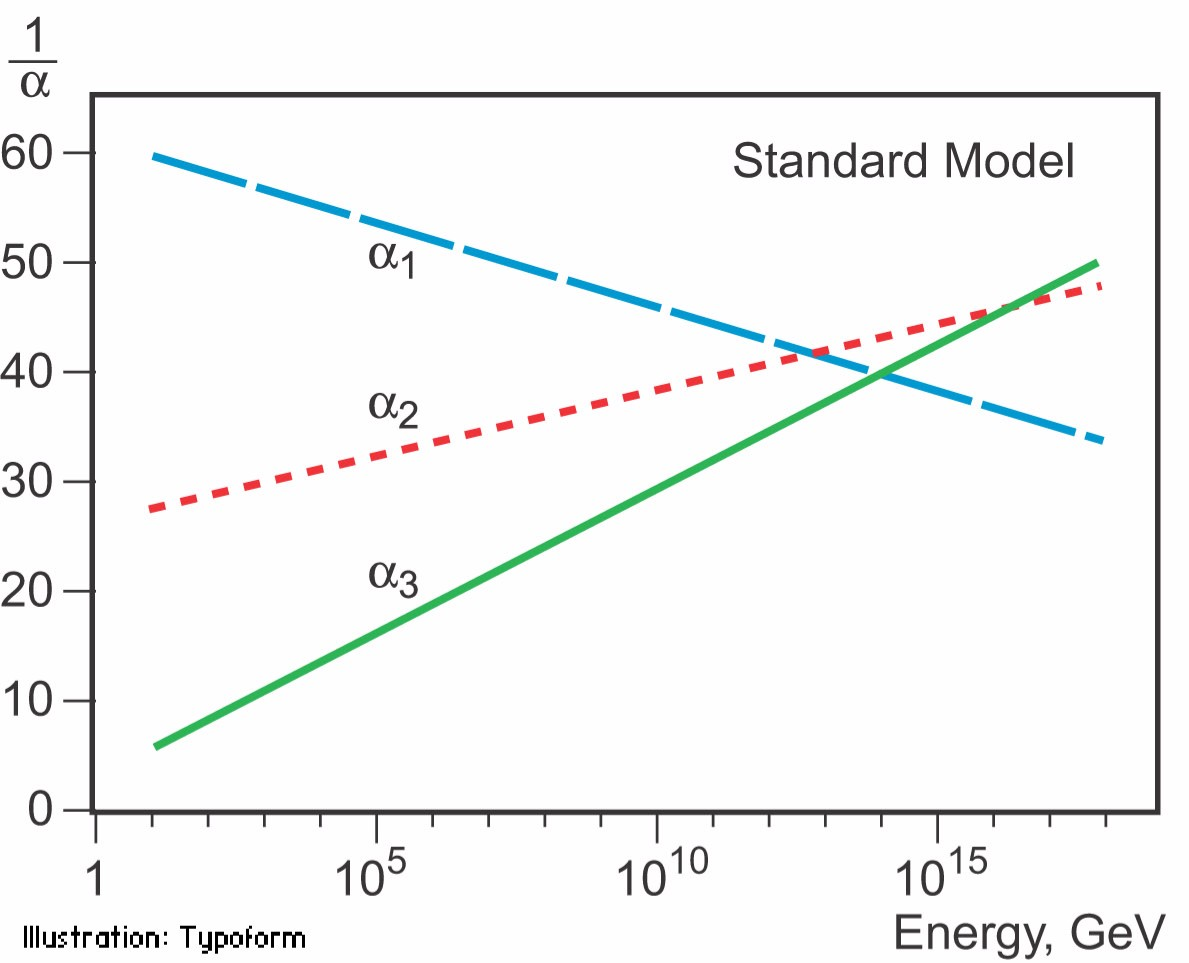
\includegraphics[width=\fullfig]{figures/unification_sm.jpg}
\caption{An approximation of the running of the coupling constants in the \acs*{SM} up to the Planck scale~\cite{unification_plot}.}
\label{fig:unification_sm}
\end{figure}


\subsection{Electroweak Physics}

The masses of the $W$ and $Z$ bosons result in significantly different processes for the weak fields than the electromagnetic field, despite their interactions being similar before symmetry breaking.
The massless photon is stable, and can propagate in a vacuum, resulting in the familiar long range interactions of electromagnetism.
The $W$ and $Z$ bosons, however, are unstable, as they have large enough masses to decay to fermions, such as the decays shown in Figure~\ref{fig:feyn_weak}.
For this reason, photons can be observed directly, while the other bosons are sufficiently short-lived (with lifetimes around 10\tsup{-25} s) that they can only be measured from their decay products.

\begin{figure}
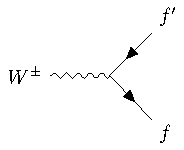
\includegraphics[width=\halffig]{figures/feyn_wdecay.pdf}
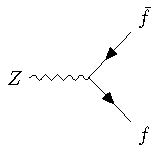
\includegraphics[width=\halffig]{figures/feyn_zdecay.pdf}\\
\caption{The Feynman diagrams representing the decays of the W and Z bosons to fermions. Here $f$ indicates a generic fermion, $\bar{f}$ its antiparticle, and $f'$ the partner of that fermion in the same generation.}
\label{fig:feyn_weak}
\end{figure}

Because the electroweak bosons interact with both quarks and leptons, they are responsible for the production of leptons in proton-proton collisions.
$Z$ bosons and photons produce pairs of opposite sign, same flavor leptons.
$W$ bosons, on the other hand, produce a single lepton and the corresponding neutrino.
The electroweak bosons also decay to hadrons by producing pairs of quarks, as shown in Figure~\ref{fig:feyn_weak}.
The $Z$~boson decays to hadrons with a branching ratio of 69.9\%, to neutrinos with 20.0\%, and to charged leptons 10.1\% of the time~\cite{pdg}.
The $W$~boson decays to hadrons with a branching ratio of 67.6\% and to leptons 32.4\%~\cite{pdg}.

\subsection{Strong Physics}
\label{sec:strong}

The phenomenology of the strong sector differs significantly from the weak sector because the gluons are massless but color charged.
Because of this, gluons can interact with each other, and contributions from multiple gluon interactions lead to a significant growth in the strength of the field at low energies.
The dependence of the field strength on the energy scale is described by renormalization, and in \ac{QCD} the coupling is only small at high energies.
Below approximately 1 \GeV, the strength of those interactions results in confinement: the interactions are so strong that when quark-antiquark pairs separate, the fields between them generate additional quarks to form color neutral bound states. 
Above around the \GeV scale, the interactions of quarks become perturbative, similar to the electroweak fields; this phenomenon is known as asymptotic freedom.

At lower energies, however, the strength of the strong interaction is so significant that the interactions of color-charged particles create additional particles until they form neutral bound-states.
This process is known as hadronization, and explains why no quarks are observed isolated in nature: they all form bound states of hadrons like protons, neutrons, and pions.
The hadronization process can produce a significant number of particles, so that a single energetic quark recoiling against another quark can generate a cascade of dozens of hadrons.
Because of the initial boost of such an energetic configuration, the resulting hadrons are collimated, and conical spray of particles often referred to as a jet.

\subsection{Proton-Proton Collisions}
\label{sec:ppcollisions}

Proton-proton collisions are a convenient way to generate high energy interactions to probe the \ac{SM} and to search for new physics.
At the energies that will be discussed in this analysis, the substructure of the protons is very important to the description of the resulting interactions.
At lowest order, protons are composed of two up quarks and one down quark, but this description is incomplete.
The actual bound state includes a chaotic sea of additional gluons and $q\bar q$ pairs, each of which carries a variable fraction of the proton's energy.
When a proton-proton collision takes place, it is these constituents that interact with each other, resulting in a highly variable collision energy even when the proton-proton energy is consistent.

The fraction of the energy carried by each constituent varies moment to moment, but can be modelled probabilistically by \acp{PDF}.
These are difficult to predict theoretically, as the \ac{QCD} calculations are non-pertur\-bative, and instead are measured in hard-scattering experiments.
They are usually represented by how often a given type of particle carries a fraction $x$ of the total proton energy.
Those fractions change significantly with the scale of the interaction, $Q$; the \acp{PDF} of proton-proton collisions at both $Q^2 = 10\ \GeV^{2}$ and $Q^2 = 10^4\ \GeV^{2}$ are shown in Figure~\ref{fig:pdfs}.

\begin{figure}
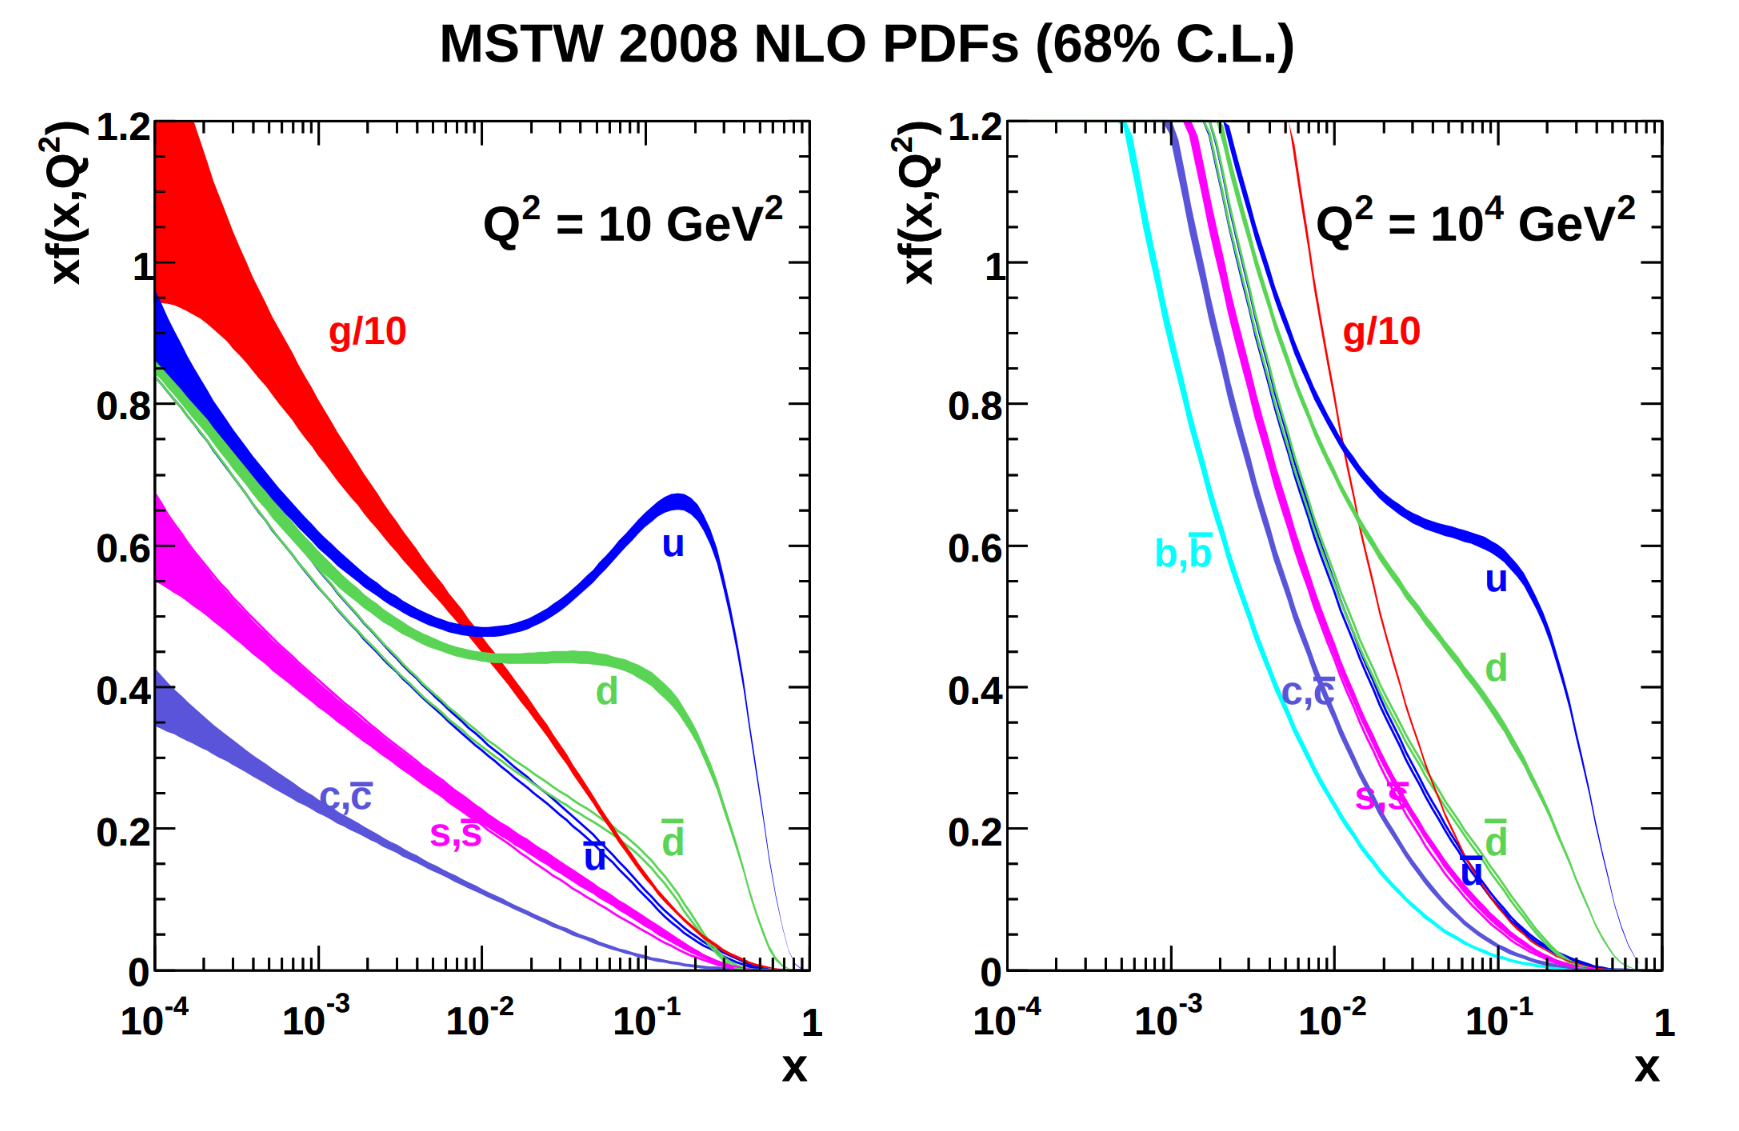
\includegraphics[width=\textwidth]{figures/pdfs.png}
\caption{The \acsp*{PDF} for proton-proton collisions at $Q^2 = 10\ \GeV^{2}$ and $Q^2 = 10^4\ \GeV^{2}$. Each shows the fraction of particles which carry a fraction $x$ of the total proton energy at the specified scale~\cite{pdfs}. The distribution for gluons is scaled by 0.1 to fit within the axis range.}
\label{fig:pdfs}
\end{figure}

The underlying \acp{PDF} of protons has important effects on the calculation of cross sections in proton-proton collisions.
Instead of specifying an exact initial momentum for the cross section calculation, in a proton-proton collision it is necessary to integrate over the contribution to a given process from the \acp{PDF} for all possible constituent particles.
The constituents are unlikely to carry the entire momentum of the proton, so the cross section for processes involving massive particle are supressed.

\subsection{Simulation}

Although the \ac{SM} provides the necessary components to model the proton-proton collisions at the \ac{LHC}, the complexity of the processes make direct predictions difficult.
The \ac{LHC} experiments rely on simulations that break down the collisions and resulting detector interactions into several steps in order to predict expected \ac{SM} and even \ac{BSM} events.
The simulation begins with a selection of two proton constituents to collide from the \acp{PDF} described in Section~\ref{sec:ppcollisions}, which fully specify the particle types and their momenta.
The initial momenta are then fed into an event generator, which calculates the cross section and predicts the final momentum using the matrix element formulation described in Section~\ref{sec:smcalc}.
This analysis uses both the \texttt{Pythia 6.4.27}~\cite{pythia6} and \texttt{MG5\_aMC@NLO}~\cite{madgraph} generators in simulated events.
The next step calculates additional processes that occur during the primary interaction, including hadronization, fragmentation, and initial state radiation. 
The result of this intial event generation is a series of particles and momentum that were produced in the collision.
These initial particle states are recorded for simulation studies, and are often referred to as truth.

These particles must then be propagated through a simulated detector geometry, where the signal they produce in the detector models can be modeled.
\texttt{Geant4}~\cite{GEANT4} provides a toolbox that describes the propagation of particles in the magnetic field as well as their interactions with the detector material.
It also simulates secondary interactions where additional particles may be produced, such as a photon interacting with the detector material and converting to two electrons.
Each particle is tracked until its energy is lost or it exits the volume of the detector, and the signals it generates in the active regions of the detector simulation are recorded.
Those signal are then converted into the expected electronic outputs of the detector in a process called digitization.
The result of this step has precisely the same format as collected data, so that both can be fed into the same reconstruction algorithms for analysis.

\section{Limitations}
\label{sec:limitations}

Despite the great success of the relatively simple \ac{SM} in describing such a broad range of emergent phenomena, it is clear that the picture it presents of the interactions of fundamental particles is incomplete.
The \ac{SM} contains concerning coincidences that suggest a more ordered underlying substructure that is not expressed in the current form.
It also fails to explain a number of cosmological measurements of the nature of matter in the universe.
These limitations suggest the need for new, \ac{BSM} physics that would provide a more complete description at higher energies.


\subsection{Theoretical Concerns}

There have been no successful integrations of the \ac{SM}'s description of the electroweak and strong forces with the description of gravity, and it is still unclear how to account for the effects of gravity at the Planck scale of approximately $10^{19}$ \GeV, where its interactions are as strong as the remaining forces.
The Planck scale is an important cutoff for the \ac{SM}, as it is clear that the \ac{SM} must break down somewhere between the current highest energy tests of the \ac{SM}, around 1 \TeV, and the Planck scale.

One example of this is the Higgs mass, which is determined by a sum of it's bare mass and the interactions in the vacuum with all massive particles.
As there must be new physics at the Planck scale to describe gravity, some of those corrections would include contributions at a scale seventeen orders of magnitude above the mass of the Higgs.
Either the bare mass of the Higgs boson precisely cancels those contributions to leave a remainder seventeen orders of magnitudes smaller, or a new theory exists at a lower scale the shields the Higgs mass from those terms.
A theory where such a unlikely cancellation of free parameters occurs is called fine-tuned, and one that is free from such cancellations is called natural.
Theories where the mass of the Higgs is natural are usually preferred, as they suggest an underlying, coherent structure.
The enormous difference in scales between the weak scale (including the Higgs mass), and the Planck scale, is often referred to as the hierarchy problem.

There is also a compelling argument that the $SU(3)\times SU(2) \times U(1)$ gauge structure of the \ac{SM} might originate from a single, unified gauge theory.
For example, it is possible to represent that gauge structure as a $SU(5)$ gauge group with only a few inconsistencies with the current implementation.
This unification is suggested by the scaling of the coupling constants for each of the forces under renormalization; they come close to converging to a single value at higher energies, as seen in Figure~\ref{fig:unification_sm}. 
An additional correction to the scaling of the coupling constants from new physics above the \TeV scale could cause them to merge into a single value at high energies. 

\subsection{Cosmological Observations}

The \ac{SM} contains a symmetry in the description of matter and antimatter that is not reflected in cosmological observations.
The processes of the standard model create or remove matter and antimatter in equal amounts, so a universe that begins with an equal quantity of each should result in a universe with an approximate\footnote{There are some processes in the standard model which can result in a small imbalance of matter and antimatter, but not at the scale observed cosmologically.} balance of matter and antimatter.
However, cosmological observations of the relative amount of each type clearly show that the directly observable mass of the universe is overwhelmingly made of matter.
As this difference is largely a difference in the generation of baryons and anti-baryons, this discrepancy is often referred to as the baryogenesis problem.

A number of astrophysical observations of large scale gravitational interactions suggest the presence of a significant amount of non-luminous matter that interacts with the normal matter only gravitationally.
The first evidence of this came from the observation of galactic rotation curves, the velocities of stars as a function of the radius from the center of a galaxy.
These can be directly predicted from the amount of matter contained within the sphere up to the radius of the star.
An estimate of velocity based only on the luminous matter in the galaxies would predict a dependence that falls off with the radius, but the observed curves show a mostly constant distribution of velocities~\cite{rotation_curves}, as seen in Figure~\ref{fig:rotational_curve}.
The higher velocities than predicted by the luminous matter can be explained by a halo of dark matter that extends significantly outside the galactic disk.

\begin{figure}
\centering
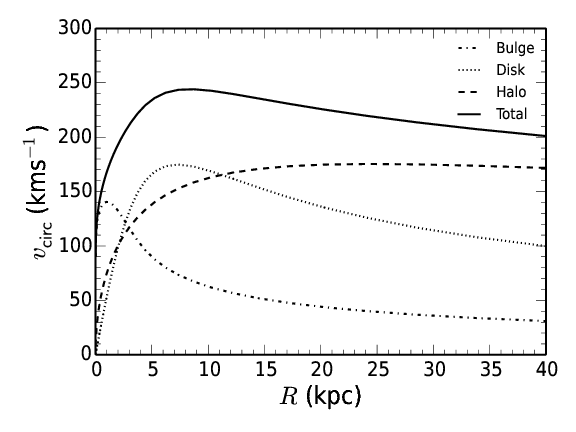
\includegraphics[width=\fullfig]{figures/rotation_curves.png}
\caption{The distribution of velocities of stars as a function of the radius from the center of the galaxy. The contributions to the velocity from the various components of matter in the galaxy are shown~\cite{rotation_curves}.}
\label{fig:rotational_curve}
\end{figure}

This dark matter accounts for a majority of the matter in the universe, and is incompatible with the matter particles predicted by the \ac{SM}.
Many observations support its existence, but there have been no direct detections of a particle which could account for the large quantity of gravitationally interacting dark matter.
The \ac{SM} would have to require a significant extension to include the particles needed to explain dark matter and the processes needed to explain the observed matter-antimatter asymmetry. 
